\documentclass[11pt]{article}

% Increase main memory size
\usepackage{etex}
\usepackage{morewrites}
\usepackage{multicol}
\usepackage{pgfplots}
\usepackage{tikz}
\usetikzlibrary{external}
\tikzexternalize[prefix=cached_models/]

\usepackage{etex}
\usepackage{morewrites}
\usepackage{enumitem}
\usepackage{float}

\listfiles

\usepackage{amsmath, amssymb, amsthm}
\usepackage{graphicx}
\usepackage{geometry}
\usepackage{array}
\usepackage{booktabs}
\usepackage{float}
\usepackage{verbatim}
\usetikzlibrary{3d}

% Page Layout
\geometry{a4paper, margin=1in}
\setlength\parindent{0pt}
\pgfplotsset{compat=1.18}

% Custom commands
\newcommand{\card}[1]{\lvert #1 \rvert}
\newcommand{\inner}[2]{\left\langle #1, #2 \right\rangle}

\title{\textbf{Vector Calculus}}
\author{}
\date{}

\begin{document}

\maketitle

\section{Euclidean space}

\subsection{Basic Concepts}

We define the \textbf{Euclidean space} $\mathbb{R}^n$, $n \geq 1$, as the set of all elements in $\mathbb{R}$:
\[ x = (x_1, x_2, \ldots, x_n) \quad \text{where } x_i \in \mathbb{R} \text{ for } i = 1, 2, \ldots, n. \]

The \textbf{Standard basis} of $\mathbb{R}^n$ is given by the vectors:
\[ e_1 = (1, 0, \ldots, 0), \quad e_2 = (0, 1, \ldots, 0), \quad \ldots, \quad e_n = (0, 0, \ldots, 1). \]

Then, any vector $x \in \mathbb{R}^n$ can be expressed as a linear combination of the standard basis vectors:
\[ x = x_1 e_1 + x_2 e_2 + \ldots + x_n e_n. \]

\subsection{Properties of Euclidean Space}
The Euclidean space $\mathbb{R}^n$ has the following properties:
\begin{itemize}
    \item \textbf{Addition:} For any $x, y \in \mathbb{R}^n$, the sum $x + y$ is defined component-wise:
    \[ x + y = (x_1 + y_1, x_2 + y_2, \ldots, x_n + y_n). \]
    \item \textbf{Scalar Multiplication:} For any scalar $\alpha \in \mathbb{R}$ and vector $x \in \mathbb{R}^n$, the product $\alpha x$ is defined as:
    \[ \alpha x = (\alpha x_1, \alpha x_2, \ldots, \alpha x_n). \]
    \item \textbf{Scalar Distributivity:} For any scalars $\alpha, \beta \in \mathbb{R}$ and vector $x \in \mathbb{R}^n$:
    \[ (\alpha + \beta)x = \alpha x + \beta x. \]
    \item \textbf{Vector Distributivity:} For any scalar $\alpha \in \mathbb{R}$ and vectors $x, y \in \mathbb{R}^n$:
    \[ \alpha(x + y) = \alpha x + \alpha y. \]
    \item \textbf{Scalar Commutativity:} For any scalars $\alpha, \beta \in \mathbb{R}$ and vector $x \in \mathbb{R}^n$:
    \[ \alpha(\beta x) = (\alpha \beta)x. \]
    \item \textbf{Multiplicative Identity:} For any vector $x \in \mathbb{R}^n$:
    \[ 1 \cdot x = x. \]
    \item \textbf{Multiplicative Zero:} For any vector $x \in \mathbb{R}^n$:
    \[ 0 \cdot x = 0. \]
\end{itemize}
\pagebreak
\subsection{Geometric Interpretation}
\begin{multicols}{2}
The Euclidean space $\mathbb{R}^n$ can be visualized as an $n$-dimensional space where each point corresponds to a vector. Given a vector $x = (x_1, x_2, \ldots, x_n)$, and a scalar $\alpha \in \mathbb{R}$, the vector $\alpha x$ represents a point that is scaled by the factor $\alpha$ in the direction of $x$:
\begin{center}
\begin{tikzpicture}
    \begin{axis}
        \addplot[->, very thick] coordinates {(0,0) (2,3)} node at (1.8,3.3) {$x$};
        \addplot[->, thick, red] coordinates {(0,0) (4,6)} node at (3.8,6.3) {$2x$};
        \addplot[->, thick, blue] coordinates {(0,0) (1,1.5)} node at (0.75,1.8) {$0.5x$};
    \end{axis}
\end{tikzpicture}
\end{center}
\end{multicols}

Given two vectors $x, y \in \mathbb{R}^n$, their sum $x + y$ represents the vector obtained by placing the tail of $y$ at the head of $x$. Similarly, the difference $x - y$ can be visualized by reversing the direction of $y$ and adding it to $x$.
\begin{center}
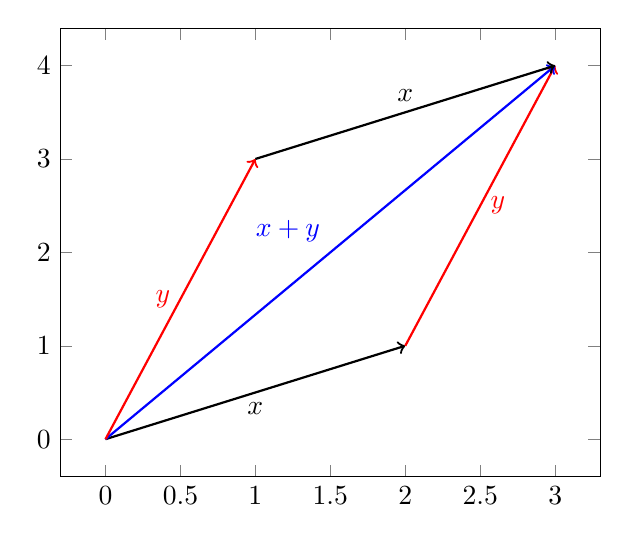
\begin{tikzpicture}
    \begin{axis}
        \addplot[->, thick] coordinates {(0,0) (2,1)} node[midway, below] {$x$};
        \addplot[->, thick, red] coordinates {(2,1) (3,4)} node[midway, right] {$y$};
        \addplot[->, thick, blue] coordinates {(0,0) (3,4)} node[midway, above left] {$x + y$};
        \addplot[->, thick, red] coordinates {(0,0) (1,3)} node[midway, left] {$y$};
        \addplot[->, thick] coordinates {(1,3) (3,4)} node[midway, above] {$x$};
    \end{axis}
\end{tikzpicture}
\hspace{0.5cm}
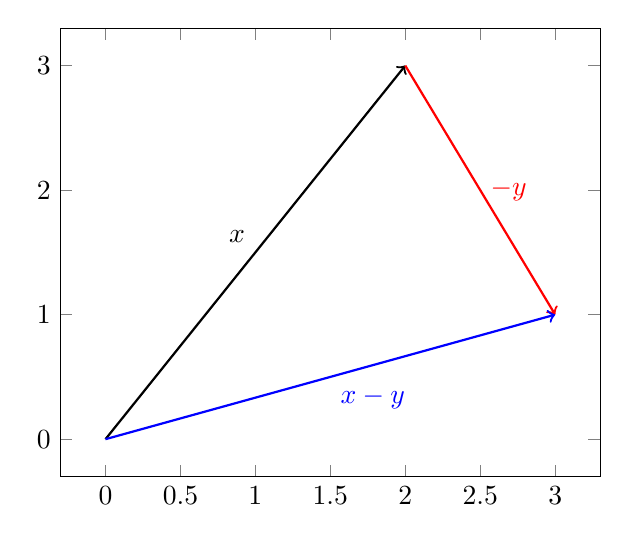
\begin{tikzpicture}
    \begin{axis}
        \addplot[->, thick] coordinates {(0,0) (2,3)} node[midway, above left] {$x$};
        \addplot[->, thick, red] coordinates {(2,3) (3,1)} node[midway, right] {$-y$};
        \addplot[->, thick, blue] coordinates {(0,0) (3,1)} node[midway, below right] {$x - y$};
    \end{axis}
\end{tikzpicture}
\end{center}

\subsection{Norm and Distance}
The Euclidian space is a \textbf{normed vector space} with the norm defined as:
\begin{align*}
\|\cdot\| : \text{ } & \mathbb{R}^n \to \mathbb{R} \\
& x \mapsto \|x\| = \sqrt{x_1^2 + x_2^2 + \ldots + x_n^2}.
\end{align*}

The norm satisfies the following properties for all $x, y \in \mathbb{R}^n$ and $\alpha \in \mathbb{R}$:
\begin{itemize}
    \item \textbf{Non-negativity:} $\|x\| \geq 0$ and $\|x\| = 0$ if and only if $x = 0$.
    \item \textbf{Scalar Multiplication:} $\|\alpha x\| = |\alpha| \|x\|$.
    \item \textbf{Triangle Inequality:} $\|x + y\| \leq \|x\| + \|y\|$.
\end{itemize}
\pagebreak
\subsubsection*{Remark}
Associated with the norm is the \textbf{distance function} $d : \mathbb{R}^n \times \mathbb{R}^n \to \mathbb{R}$ defined by:
\[ d(x, y) = \|x - y\|. \]
The distance function satisfies the following properties for all $x, y, z \in \mathbb{R}^n$:
\begin{itemize}
    \item \textbf{Non-negativity:} $d(x, y) \geq 0$ and $d(x, y) = 0$ if and only if $x = y$.
    \item \textbf{Symmetry:} $d(x, y) = d(y, x)$.
    \item \textbf{Triangle Inequality:} $d(x, z) \leq d(x, y) + d(y, z)$.
\end{itemize}

\subsubsection{Norms in $\mathbb{R}^3$}
\begin{multicols}{2}
In $\mathbb{R}^3$, the norm of a vector $x = (x_1, x_2, x_3)$ is given by:
\[ \|x\| = d(O, x) = OB^2 + x_3^2 = \sqrt{x_1^2 + x_2^2 + x_3^2}, \]
where $O$ is the origin and $B$ is the projection of $x$ onto the $xy$-plane:
\begin{center}
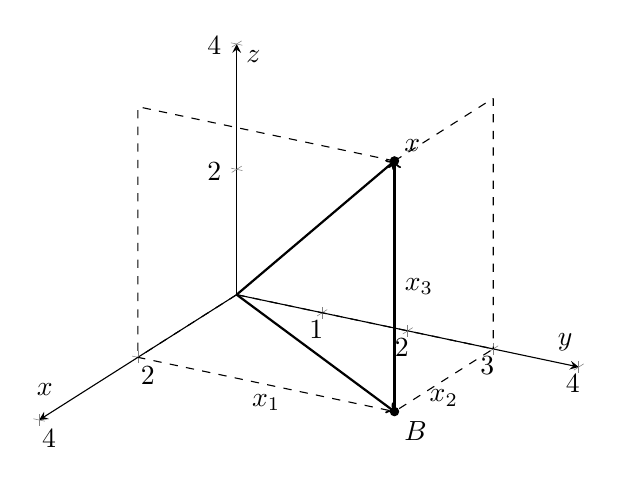
\begin{tikzpicture}
    \begin{axis}[view={120}{30}, axis lines=center, xlabel=$x$, ylabel=$y$, zlabel=$z$, xmax=4, ymax=4, zmax=4]
        \addplot3[->, thick] coordinates {(0,0,0) (2,3,4)};
        \addplot3[dashed] coordinates {(2,3,0) (2,3,4)};
        \addplot3[->, thick] coordinates {(0,0,0) (2,3,0)};   
        \addplot3[->, thick] coordinates {(2,3,0) (2,3,4)} node[midway, right] {$x_3$};
        \draw[dashed] (axis cs:0,0,0) -- (axis cs:2,0,0) -- (axis cs:2,3,0) node[midway, below] {$x_1$};
        \draw[dashed] (axis cs:0,0,0) -- (axis cs:0,3,0) -- (axis cs:2,3,0) node[midway, below] {$x_2$};
        \draw[dashed] (axis cs:2,3,4) -- (axis cs:0,3,4) -- (axis cs:0,3,0);
        \draw[dashed] (axis cs:2,3,4) -- (axis cs:2,0,4) -- (axis cs:2,0,0);
        \draw[fill] (axis cs:2,3,4) circle [radius=1.5pt] node[above right] {$x$};
        \draw[fill] (axis cs:2,3,0) circle [radius=1.5pt] node[below right] {$B$};
    \end{axis}
\end{tikzpicture}
\end{center}
\end{multicols}

\subsection{Inner or Scalar Product}
Let $x, y \in \mathbb{R}^n$. The \textbf{inner product} (or \textbf{scalar product}) of $x$ and $y$ is defined as:
\[ x \cdot y = \inner{x}{y} = x_1 y_1 + x_2 y_2 + \ldots + x_n y_n. \]

The inner product satisfies the following properties for all $x, y, z \in \mathbb{R}^n$ and $\alpha \in \mathbb{R}$:
\begin{itemize}
    \item \textbf{Positive Definite:} $x \cdot x \geq 0$ and $x \cdot x = 0$ if and only if $x = 0$.
    \item \textbf{Symmetry:} $x \cdot y = y \cdot x$.
    \item \textbf{Bilinear Form:} $\inner{\lambda x + \mu y}{z} = \lambda \inner{x}{z} + \mu \inner{y}{z}$ for all $\lambda, \mu \in \mathbb{R}$.
\end{itemize}

\subsection{Cauchy-Schwarz Inequality}
For any vectors $x, y \in \mathbb{R}^n$, the Cauchy-Schwarz inequality states that:
\[ |x \cdot y| \leq \|x\| \|y\|. \]
Equality holds if and only if $x$ and $y$ are linearly dependent.
\pagebreak
\begin{proof}
    If $y = \lambda x$ for some $\lambda \in \mathbb{R}$, then:
    \[ |x \cdot y| = |x \cdot (\lambda x)| = |\lambda| \|x\|^2 = \|x\| \|\lambda x\|. \]
    If $x$ and $y$ are linearly independent, consider the vector $z = \lambda x + y$ for some $\lambda \in \mathbb{R}$. Then:
    \[ 0 \leq \inner{z}{z} = \|z\|^2 = \inner{\lambda x + y}{\lambda x + y}. \]
    Expanding this, we have:
    \[ \|z\|^2 = \lambda^2 \|x\|^2 + 2\lambda \inner{x}{y} + \|y\|^2, \]
    which is a quadratic function in $\lambda$.
    For $f(\lambda) \geq 0$ for all $\lambda$, the discriminant must be non-positive:
    \[ (2\inner{x}{y})^2 - 4\|x\|^2 \|y\|^2 \leq 0. \]
    Simplifying, we get:
    \[ 4\inner{x}{y}^2 \leq 4\|x\|^2 \|y\|^2, \]
    which leads to:
    \[ |x \cdot y| \leq \|x\| \|y\|. \]
\end{proof}

\subsection{Theorem: Inner Product and Norm}
For any vectors $x, y \in \mathbb{R}^n$, the following relation holds:
\[ \inner{x}{y} = \|x\| \|y\| \cos \theta, \]
where $\theta$ is the angle between the vectors $x$ and $y$.

\begin{proof}
    \begin{multicols}{2}
    Consider the vectors $x$ and $y$ in $\mathbb{R}^2$ . Let the angle between $x$ and the positive $x$-axis be $\alpha$, and the angle between $y$ and the positive $x$-axis be $\beta$. Then, the angle between $x$ and $y$ is given by $\theta = \beta - \alpha$. We have:
        \[x_1 = \|x\| \cos \alpha, \quad x_2 = \|x\| \sin \alpha,\]
        \[y_1 = \|y\| \cos \beta, \quad y_2 = \|y\| \sin \beta.\]
    \vspace{2cm}
    \begin{center}
        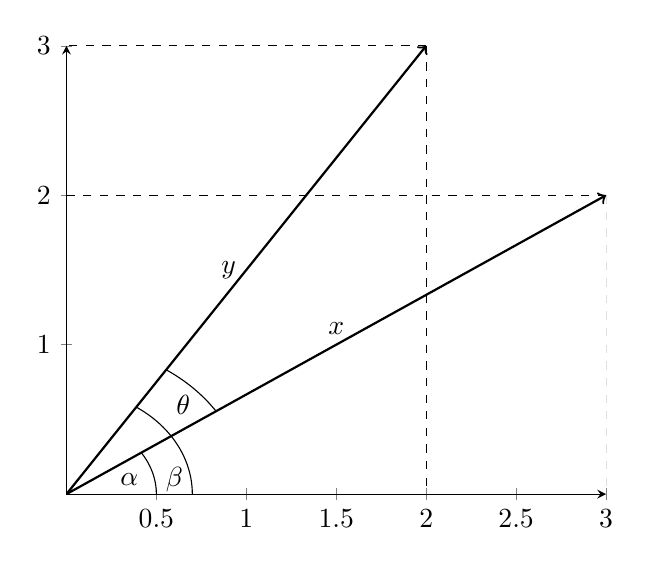
\begin{tikzpicture}
            \begin{axis}[axis lines=middle]
                \addplot[->, thick] coordinates {(0,0) (3,2)} node[midway, above] {$x$};
                \addplot[->, thick] coordinates {(0,0) (2,3)} node[midway, left] {$y$};
                \addplot[dashed] coordinates {(3,2) (3,0)};
                \addplot[dashed] coordinates {(2,3) (2,0)};
                \addplot[dashed] coordinates {(2,3) (0,3)};
                \addplot[dashed] coordinates {(3,2) (0,2)};
                \addplot[domain=0:33.69] ({0.5*cos(x)}, {0.5*sin(x)}) node at (0.35,0.1) {$\alpha$};
                \addplot[domain=0:56.31] ({0.7*cos(x)}, {0.7*sin(x)}) node at (0.6,0.1) {$\beta$};
                \addplot[domain=33.69:56.31] ({1.0*cos(x)}, {1.0*sin(x)}) node at (0.65,0.6) {$\theta$};
            \end{axis}
        \end{tikzpicture}
    \end{center}
\end{multicols}

Therefore, the inner product is:
\begin{align*}
\inner{x}{y} & = x_1 y_1 + x_2 y_2 \\
& = \|x\| \cos \alpha \cdot \|y\| \cos \beta + \|x\| \sin \alpha \cdot \|y\| \sin \beta \\
& = \|x\| \|y\| (\cos \alpha \cos \beta + \sin \alpha \sin \beta) \\
& = \|x\| \|y\| \cos(\beta - \alpha) \\
& = \|x\| \|y\| \cos \theta.
\end{align*}
\end{proof}

\subsubsection*{Remark}
From the theorem, we can derive the formula for the angle $\theta$ between two vectors $x$ and $y$:
\[ \theta = \arccos \left( \frac{\inner{x}{y}}{\|x\| \|y\|} \right). \]

Note that if $x \perp y$ (i.e., $x$ is perpendicular to $y$), then $\inner{x}{y} = 0$ and thus $\theta = \frac{\pi}{2}$.

\subsubsection*{Examples}
$C(a, b)$ is the set of continuous functions on the interval $(a, b)$. For any $f, g \in C(a, b)$, we define the inner product as:
\[ \inner{f}{g} = \int_a^b f(x) g(x) \, dx. \]

We can add a weighted inner product as follows:
\[ \inner{f}{g}_w = \int_a^b f(x) g(x) w(x) \, dx, \]
where $w(x)$ is a weight function such as $w(x) = e^{-x}$ or $w(x) = 1/x^2$.

We might as well use the family of \textbf{orthogonal functions}:
\[\{\cos nx , \sin nx \mid n = 0, 1, 2, \ldots\} \quad \text{Fourier family}.\]
\[0 = \int^{2\pi}_0 \cos nx \sin nx \, dx = \int^{2\pi}_0 \cos nx \cos mx \, dx = \int^{2\pi}_0 \sin nx \sin mx \, dx, \quad n \neq m.\]

\subsection{Vector Product in $\mathbb{R}^3$}
Let $x = (x_1, x_2, x_3)$ and $y = (y_1, y_2, y_3)$ be two vectors in $\mathbb{R}^3$. The \textbf{vector product} (or \text{cross product}) of $x$ and $y$ is defined as:
\[ x \times y = \begin{vmatrix}
\mathbf{i} & \mathbf{j} & \mathbf{k} \\
x_1 & x_2 & x_3 \\
y_1 & y_2 & y_3
\end{vmatrix} = \begin{vmatrix}
x_2 & x_3 \\
y_2 & y_3
\end{vmatrix} \mathbf{i} - \begin{vmatrix}
x_1 & x_3 \\
y_1 & y_3
\end{vmatrix} \mathbf{j} + \begin{vmatrix}
x_1 & x_2 \\
y_1 & y_2
\end{vmatrix} \mathbf{k}, \]
where $\mathbf{i}, \mathbf{j}, \mathbf{k}$ are the standard unit vectors in $\mathbb{R}^3$.

\subsubsection{Geometric Interpretation}
To visualize the vector product, consider the triple product $a \cdot (b \times c)$, which represents the volume of the parallelepiped formed by the vectors $a, b,$ and $c$:
\[a \cdot (b \times c) = (a_1, a_2, a_3) \cdot \begin{vmatrix}
b_2 & b_3 \\
c_2 & c_3
\end{vmatrix} \mathbf{i} - \begin{vmatrix}
b_1 & b_3 \\
c_1 & c_3
\end{vmatrix} \mathbf{j} + \begin{vmatrix}
b_1 & b_2 \\
c_1 & c_2
\end{vmatrix} \mathbf{k} = \begin{vmatrix}
a_1 & a_2 & a_3 \\
b_1 & b_2 & b_3 \\
c_1 & c_2 & c_3
\end{vmatrix}.\]

If $a \in \text{span}\{b, c\}$, then the volume is zero, indicating that the vectors are coplanar.
\begin{center}
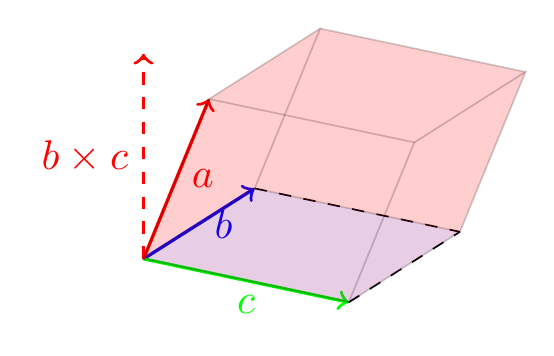
\begin{tikzpicture}[scale=1.5]
    \begin{axis}[view={120}{30}, axis lines=none, xlabel=$x$, ylabel=$y$, zlabel=$z$, xmax=5, ymax=5, zmax=5]
        % Vectors b and c in the xy-plane
        \addplot3[->, thick, blue] coordinates {(0,0,0) (-3,0,0)} node[midway, right] {$b$};
        \addplot3[->, thick, green] coordinates {(0,0,0) (0,2,0)} node[midway, below] {$c$};
        \addplot3[dashed] coordinates {(-3,0,0) (-3,2,0)};
        \addplot3[dashed] coordinates {(0,2,0) (-3,2,0)};
        \addplot3[->, dashed, red, thick] coordinates {(0,0,0) (0,0,3)} node[midway, left] {$b \times c$};
        % Vector a above the xy-plane
        \addplot3[->, thick, red] coordinates {(0,0,0) (1,1,3)} node[midway, right] {$a$};
        % Parallelepiped edges
        \draw[fill=blue, opacity=0.1] (0,0,0) -- (-3,0,0) -- (-3,2,0) -- (0,2,0) -- cycle;
        \draw[fill=red, opacity=0.1] (0,0,0) -- (1,1,3) -- (-2,1,3) -- (-3,0,0) -- cycle;
        \draw[fill=red, opacity=0.1] (0,0,0) -- (1,1,3) -- (1,3,3) -- (0,2,0) -- cycle;
        \draw[fill=red, opacity=0.1] (-3,0,0) -- (-2,1,3) -- (-2,3,3) -- (-3,2,0) -- cycle;
        \draw[fill=red, opacity=0.1] (0,2,0) -- (1,3,3) -- (-2,3,3) -- (-3,2,0) -- cycle;
        \draw[fill=red, opacity=0.1] (1,1,3) -- (-2,1,3) -- (-2,3,3) -- (1,3,3) -- cycle;
    \end{axis}
\end{tikzpicture}
\end{center}

Also, 
\[\|b \times c\|^2 = \begin{vmatrix}
b_2 & b_3 \\
c_2 & c_3
\end{vmatrix}^2 + \begin{vmatrix}
b_1 & b_3 \\
c_1 & c_3
\end{vmatrix}^2 + \begin{vmatrix}
b_1 & b_2 \\
c_1 & c_2
\end{vmatrix}^2 = (b_2 c_3 - b_3 c_2)^2 + (b_1 c_3 - b_3 c_1)^2 + (b_1 c_2 - b_2 c_1)^2 = \]
\[= (b_1^2 + b_2^2 + b_3^2)(c_1^2 + c_2^2 + c_3^2) - (b_1 c_1 + b_2 c_2 + b_3 c_3)^2 = \|b\|^2 \|c\|^2 - (b \cdot c)^2 = \|b\|^2 \|c\|^2 \sin^2 \theta.\]

Thus, we have:
\[\|b \times c\| = \|b\| \|c\| \sin \theta,\]
where $\theta$ is the angle between vectors $b$ and $c$. This represents the area of the parallelogram formed by $b$ and $c$.
\begin{center}
    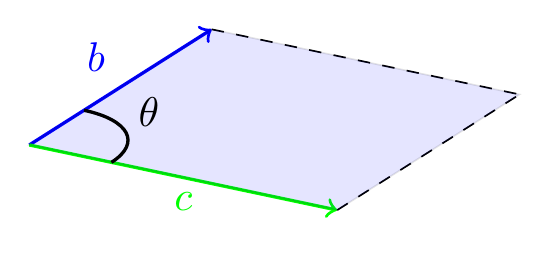
\begin{tikzpicture}[scale=1.5]
        \begin{axis}[view={120}{30}, axis lines=none, xlabel=$x$, ylabel=$y$, zlabel=$z$, xmax=5, ymax=5, zmax=4]
        \addplot3[->, thick, blue] coordinates {(0,0,0) (-8,0,0)} node[midway, above left] {$b$};
        \addplot3[->, thick, green] coordinates {(0,0,0) (0,3,0)} node[midway, below] {$c$};
        \addplot3[dashed] coordinates {(-8,0,0) (-8,3,0)};
        \addplot3[dashed] coordinates {(0,3,0) (-8,3,0)};
        \draw[fill=blue, opacity=0.1] (0,0,0) -- (-8,0,0) -- (-8,3,0) -- (0,3,0) -- cycle;
        \draw[thick] (0,0.8,0) arc[start angle=90, end angle=180,x radius=2.4,y radius=0.8];
        \node at (-3,0.5,0) {$\theta$};
        \end{axis}
    \end{tikzpicture}
\end{center}
\pagebreak
\section{Level Curves}
Let $A \subset \mathbb{R}^n$ be a subset of $\mathbb{R}^n$ and let $f : A \to \mathbb{R}$ be a real-valued function defined on $A$. For any constant $c \in \mathbb{R}$, the \textbf{level set} of $f$ corresponding to the value $c$ is defined as:
\[ L_c = \{ x \in A \mid f(x) = c \}. \]

In the case where $n = 2$, the level sets are called \textbf{level curves} or \textbf{contour lines}. In the case where $n = 3$, the level sets are called \textbf{level surfaces}.

\subsubsection*{Example (Chapter 12, Ex 3)}
Consider the function $f : \mathbb{R}^2 \to \mathbb{R}$ defined by:
\[ f(x, y) = xy. \]
The level curves of $f$ for different values of $c$ are given by:
\begin{itemize}
    \item For $c = -1$: $L_{-1} = \{ (x, y) \in \mathbb{R}^2 \mid xy = -1 \}$.
    \item For $c = 1$: $L_1 = \{ (x, y) \in \mathbb{R}^2 \mid xy = 1 \}$.
    \item For $c = 3$: $L_3 = \{ (x, y) \in \mathbb{R}^2 \mid xy = 3 \}$.
\end{itemize}

\subsection{Graph of a Function}
The \textbf{graph} of a function $f : A \to \mathbb{R}$ is defined as the set of points in $\mathbb{R}^{n+1}$ given by:
\[ G_f = \{ (x, f(x)) \mid x \in A \}. \]

If for instance, $f : \mathbb{R}^2 \to \mathbb{R}$, then the graph of $f$ is a surface in $\mathbb{R}^3$.
\begin{center}
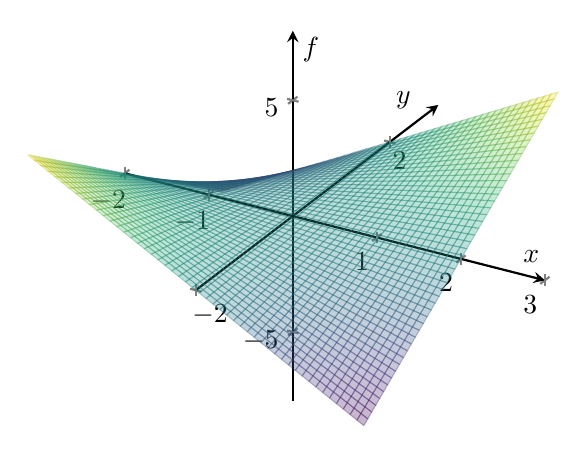
\begin{tikzpicture}
    \begin{axis}[view={30}{30}, axis lines=center, xlabel=$x$, ylabel=$y$, zlabel=$f$, xmax=3, ymax=3, zmax=8, zmin=-8, width=10cm, height=10cm, axis line style={thick}, tick style={thick}]
        \addplot3[surf, domain=-2:2, y domain=-2:2, opacity=0.3, colormap/viridis, samples=50] {x*y};
    \end{axis}
\end{tikzpicture}
\hspace{1cm}
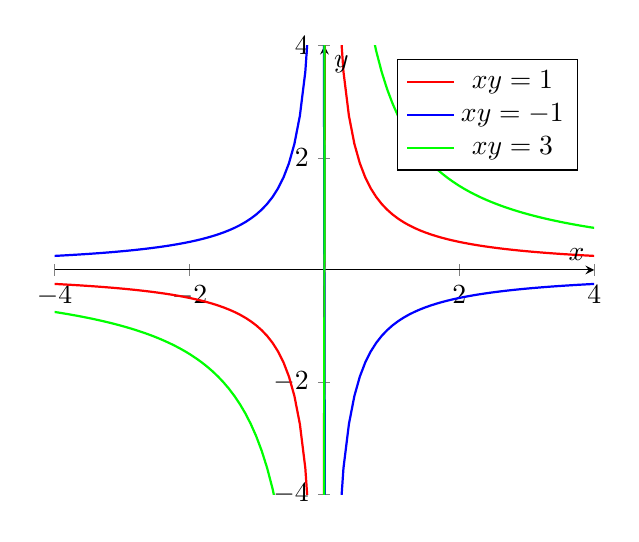
\begin{tikzpicture}
    \begin{axis}[axis lines=middle, xlabel=$x$, ylabel=$y$, xmax=4, ymax=4, xmin=-4, ymin=-4, legend pos=north east]
        \addplot[thick, domain=-4:4, samples=100, red] {1/x};
        \addplot[thick, domain=-4:4, samples=100, blue] {-1/x};
        \addplot[thick, domain=-4:4, samples=100, green] {3/x};
        \legend{$xy=1$, $xy=-1$, $xy=3$}
    \end{axis}
\end{tikzpicture}
\end{center}

\subsubsection*{Remark}
Level sets $F : U \subset \mathbb{R}^n \to \mathbb{R}^m$; $U$ open set:
\[ F^{-1}(c) = \{ x \in U \mid F(x) = c \}, \quad c = (c_1, c_2, \ldots, c_m) \]

In terms of the coordinate functions $F = (f_1, f_2, \ldots, f_m)$, we have:
\[ F(x)(c), \text{ for } x \in \mathbb{R}^n \implies f_i(x_1, x_2, \ldots, x_n) = c_i, \quad i = 1, 2, \ldots, m. \]

Hence,
\[ F^{-1}(c) = \bigcap_{i=1}^m \{ x \in \mathbb{R}^n \mid f_i(x) = c_i \}. \]

\subsubsection*{Example}
Let $F : \mathbb{R}^3 \to \mathbb{R}^2$ be defined by:
\[ F(x, y, z) = (x^2 + y^2 + z^2 - 1, 2x^2 + 2y^2 - 1). \]
The coordinate functions are:
\begin{align*}
f^{-1}_1(0) = \{(x,y,z) \in \mathbb{R}^3 \mid x^2 + y^2 + z^2 - 1 & = 0\}, \\
f^{-1}_2(0) = \{(x,y,z) \in \mathbb{R}^3 \mid 2x^2 + 2y^2 - 1 & = 0\}.
\end{align*}

To find the level set we solve the system of equations:
\begin{align*}
x^2 + y^2 + z^2 - 1 & = 0, \\
2x^2 + 2y^2 - 1 & = 0.
\end{align*}
\begin{multicols}{2}
From the second equation, we have:
\[ x^2 + y^2 = \frac{1}{2}. \]
Substituting this into the first equation gives:
\[ \frac{1}{2} + z^2 - 1 = 0 \implies z^2 = \frac{1}{2} \implies z = \pm \frac{1}{\sqrt{2}}. \]
Thus, the level set $F^{-1}(0)$ is the intersection of the sphere $x^2 + y^2 + z^2 = 1$ and the cylinder $2x^2 + 2y^2 = 1$.
\begin{center}
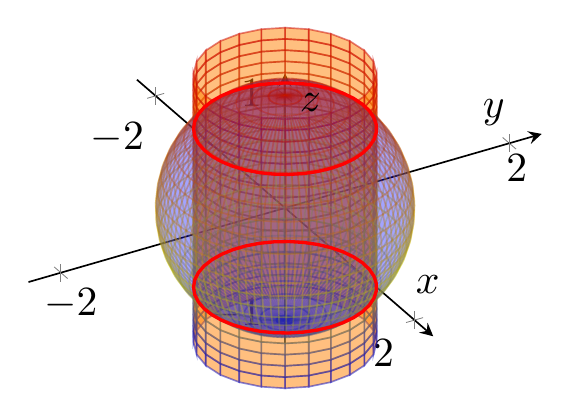
\begin{tikzpicture}[scale=1.5]
    \begin{axis}[
        view={60}{30},
        axis lines=center,
        axis equal,
        xlabel=$x$, ylabel=$y$, zlabel=$z$,
        xmin=-1.2, xmax=1.2, 
        ymin=-1.2, ymax=1.2, 
        zmin=-1.2, zmax=1.2,
    ]
        % Cylinder
        \addplot3[surf, domain=0:360, y domain=-1.2:1.2, opacity=0.5, color=orange, samples=25, z buffer=sort] 
        ({(1/sqrt(2))*cos(x)}, {(1/sqrt(2))*sin(x)}, {y});

        % Sphere
        \addplot3[surf, domain=0:360, y domain=0:180, opacity=0.2, color=blue, samples=50, z buffer=sort] 
        ({cos(y)*sin(x)}, {sin(y)*sin(x)}, {cos(x)});
        
        % Intersection curves
        \addplot3[thick, red, domain=0:360, samples=40] 
        ({(1/sqrt(2))*cos(x)}, {(1/sqrt(2))*sin(x)}, {1/sqrt(2)});
        \addplot3[thick, red, domain=0:360, samples=40] 
        ({(1/sqrt(2))*cos(x)}, {(1/sqrt(2))*sin(x)}, {-1/sqrt(2)});

    \end{axis}
\end{tikzpicture}
\end{center}
\end{multicols}

\subsubsection*{Remarks}
\begin{itemize}
    \item There is a connection between level sets and graphs. Firstly, the graph of a function $f : A \subset \mathbb{R}^n \to \mathbb{R}$ can be viewed as the level set of the function $F : A \times \mathbb{R} \to \mathbb{R}$ defined by:
        \[ F : U \subset \mathbb{R}^n \to \mathbb{R}^m, \quad F(x, z) = f(x) - z. \]

    \item The level curves allow us to draw tri-dimensional surfaces on a two-dimensional plane. 
    \item The distance between two level curves (they can never intersect) gives us information about the steepness of the surface. If the level curves are close together, the surface is steep; if they are far apart, the surface is flat.
\end{itemize}

\pagebreak

\section{Limits of Functions}
Let $f : \mathbb{R}^n \to \mathbb{R}^m$ be a function, and let $a \in \mathbb{R}^n$ be a point in its domain. We say that the limit of $f(x)$ as $x$ approaches $a$ is $L \in \mathbb{R}^m$, denoted by:
\[ \lim_{x \to a} f(x) = L, \]
if for every $\epsilon > 0$, there exists a $\delta > 0$ such that for all $x \in \mathbb{R}^n$ satisfying $0 < \|x - a\| < \delta$, we have:
\[ \|f(x) - L\| < \epsilon. \]

\subsection{Methods to Compute Limits}
\begin{enumerate}
    \item \textbf{Applying the Definition:} We must prove that for every $\epsilon > 0$, there exists a $\delta > 0$ such that 
        \[ 0 < (x, y) - (a, b) < \delta \implies |f(x, y) - L| < \epsilon. \]
    \item \textbf{Iterative limits:} 
        \[\lim_{x \to a} \left( \lim_{y \to b} f(x, y) \right) \neq \lim_{y \to b} \left( \lim_{x \to a} f(x, y) \right).\]
        This gives non-existence of the limit, so we cannot prove existence by this method.
    \item \textbf{Following families of functions:} If we can find two different paths approaching the same point that yield different limit values, then the limit does not exist.
\end{enumerate}

\end{document}